\section{KYC process}

\begin{figure}[h!]
  \begin{sequencediagram}
    \newinst{wallet}{\shortstack{Customer \\
      \\ 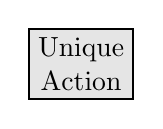
\begin{tikzpicture}
        \node [fill=gray!20,draw=black,thick,align=center] { Unique \\ Action};
      \end{tikzpicture}
    }}
    \newinst[2]{exchange}{\shortstack{Taler (exchange) \\
       \\ \begin{tikzpicture}[shape aspect=.5]
        \tikzset{every node/.style={cylinder,shape border rotate=90, draw,fill=gray!25}}
        \node at (1.5,0) {\shortstack{{{\tiny Database}}}};
       \end{tikzpicture}
    }}
    \newinst[2]{kyc}{\shortstack{KYC provider \\
       \\ \begin{tikzpicture}[shape aspect=.5]
        \tikzset{every node/.style={cylinder,shape border rotate=90, draw,fill=gray!25}}
        \node at (1.5,0) {\shortstack{{{\tiny Database}}}};
       \end{tikzpicture}
    }}

    \postlevel
    \mess[0]{wallet}{{Initial action}}{exchange}
    \begin{callself}{exchange}{Establish KYC requirement}{}
    \end{callself}
    \mess[0]{exchange}{Request new KYC process}{kyc}
    \mess[0]{kyc}{{Process identifier (PI)}}{exchange}
    \mess[0]{exchange}{{KYC required (PI)}}{wallet}
    \mess[0]{wallet}{{KYC start (PI)}}{kyc}
    \mess[0]{kyc}{{Request identity documentation}}{wallet}
    \mess[0]{wallet}{{Upload identity documentation}}{kyc}
    \begin{callself}{kyc}{Validate documentation}{}
    \end{callself}
    \mess[0]{kyc}{{Share documentation (PI)}}{exchange}
    \mess[0]{kyc}{{Confirm completion}}{wallet}
    \mess[0]{wallet}{{Retry action}}{exchange}
\end{sequencediagram}
  \caption{Deposit interactions between customer, Taler exchange (payment
    service provider) and external KYC provider.  The process can be
    triggered by various {\em actions} described in Chapter~\ref{chap:triggers}.}
  \label{fig:proc:kyc}
\end{figure}

At the beginning of the KYC process, the user needs to specify whether they
are an {\bf individual} or a {\bf business}.\footnote{ In pratice, we expect
most wallet-users to be individuals, but in principle a wallet could be owned
by a business.}  This then determines which types of attributes are collected
in the KYC process (Table~\ref{table:proc:kyc:individual} vs.
Table~\ref{table:proc:kyc:business}).

\begin{table}
  \caption{Information collected for individuals}
  \label{table:proc:kyc:individual}
  \begin{center}
    \begin{tabular}{l|c|r}
      {\bf Type}                 & {\bf Required}    & {\bf Example} \\ \hline \hline
      Surname                    & yes        & Mustermann \\
      First name(s)              & yes        & Max \\
      Date of birth              & yes        & 1.1.1980 \\
      Nationality                & yes        & Swiss \\
      Actual address of domicile & yes        & Seestrasse 3, 8008 Zuerich \\
      Phone number               & no         & +41-123456789 \\
      E-mail                     & no         & me@example.com \\
      Identification document    & yes        & JPG image \\
  \end{tabular}
  \end{center}
\end{table}

\begin{table}
  \caption{Information collected for businesses}
  \label{table:proc:kyc:business}
  \begin{center}
    \begin{tabular}{l|c|r}
      {\bf Type}                      & {\bf Required} & {\bf Example}        \\ \hline \hline
      Company name                    & yes        & Mega AG \\
      Registered office               & yes        & Seestrasse 4, 8008 Zuerich \\
      Company identification document & yes        & PDF file \\ \hline
      Contact person name             & yes        & Max Mustermann \\
      Phone number                    & no         & +41-123456789  \\
      E-mail                          & yes        & me@example.com \\
      Identification document         & yes        & JPG image \\
      Date of birth                   & yes        & 1.1.1980  \\
      Nationality                     & yes        & Swiss     \\ \hline
      Power of attorney arrangement   & yes        & PDF file  \\
  \end{tabular}
  \end{center}
\end{table}
